%
% This is the LaTeX template file for lecture notes for EE 382C/EE 361C.
%
% To familiarize yourself with this template, the body contains
% some examples of its use.  Look them over.  Then you can
% run LaTeX on this file.  After you have LaTeXed this file then
% you can look over the result either by printing it out with
% dvips or using xdvi.
%
%the  This template is based on the template for Prof. Sinclair's CS 270.

\documentclass[twoside]{article}
\usepackage{graphics}
\usepackage{tikz}
\usepackage{float}
\usepackage{amsmath}
\usepackage[]{algorithm2e}
\usetikzlibrary{arrows,automata}
\usetikzlibrary{arrows,matrix,positioning}
\usepackage[latin1]{inputenc}
\usetikzlibrary{graphs,graphs.standard}
\setlength{\oddsidemargin}{0.25 in}
\setlength{\evensidemargin}{-0.25 in}
\setlength{\topmargin}{-0.6 in}
\setlength{\textwidth}{6.5 in}
\setlength{\textheight}{8.5 in}
\setlength{\headsep}{0.75 in}
\setlength{\parindent}{0 in}
\setlength{\parskip}{0.1 in}

%
% The following commands set up the lecnum (lecture number)
% counter and make various numbering schemes work relative
% to the lecture number.
%
\newcounter{lecnum}
\renewcommand{\thepage}{\thelecnum-\arabic{page}}
\renewcommand{\thesection}{\thelecnum.\arabic{section}}
\renewcommand{\theequation}{\thelecnum.\arabic{equation}}
\renewcommand{\thefigure}{\thelecnum.\arabic{figure}}
\renewcommand{\thetable}{\thelecnum.\arabic{table}}

%
% The following macro is used to generate the header.
%
\newcommand{\lecture}[4]{
   \pagestyle{myheadings}
   \thispagestyle{plain}
   \newpage
   \setcounter{lecnum}{#1}
   \setcounter{page}{1}
   \noindent
   \begin{center}
   \framebox{
      \vbox{\vspace{2mm}
    \hbox to 6.28in { {\bf EE 382V: Distributed Systems 
                        \hfill Fall 2017} }
       \vspace{4mm}
       \hbox to 6.28in { {\Large \hfill Lecture #1: #2  \hfill} }
       \vspace{2mm}
       \hbox to 6.28in { {\it Lecturer: #3 \hfill Scribe: #4} }
      \vspace{2mm}}
   }
   \end{center}
   \markboth{Lecture #1: #2}{Lecture #1: #2}
   %{\bf Disclaimer}: {\it These notes have not been subjected to the
   %usual scrutiny reserved for formal publications.  They may be distributed
   %outside this class only with the permission of the Instructor.}
   \vspace*{4mm}
}

%
% Convention for citations is authors' initials followed by the year.
% For example, to cite a paper by Leighton and Maggs you would type
% \cite{LM89}, and to cite a paper by Strassen you would type \cite{S69}.
% (To avoid bibliography problems, for now we redefine the \cite command.)
% Also commands that create a suitable format for the reference list.
\renewcommand{\cite}[1]{[#1]}
\def\beginrefs{\begin{list}%
        {[\arabic{equation}]}{\usecounter{equation}
         \setlength{\leftmargin}{2.0truecm}\setlength{\labelsep}{0.4truecm}%
         \setlength{\labelwidth}{1.6truecm}}}
\def\endrefs{\end{list}}
\def\bibentry#1{\item[\hbox{[#1]}]}

%Use this command for a figure; it puts a figure in wherever you want it.
%usage: \fig{NUMBER}{SPACE-IN-INCHES}{CAPTION}
\newcommand{\fig}[3]{
			\vspace{#2}
			\begin{center}
			Figure \thelecnum.#1:~#3
			\end{center}
	}
% Use these for theorems, lemmas, proofs, etc.
\newtheorem{theorem}{Theorem}[lecnum]
\newtheorem{lemma}[theorem]{Lemma}
\newtheorem{proposition}[theorem]{Proposition}
\newtheorem{claim}[theorem]{Claim}
\newtheorem{corollary}[theorem]{Corollary}
\newtheorem{definition}[theorem]{Definition}
\newenvironment{proof}{{\bf Proof:}}{\hfill\rule{2mm}{2mm}}

% **** IF YOU WANT TO DEFINE ADDITIONAL MACROS FOR YOURSELF, PUT THEM HERE:

\begin{document}
%FILL IN THE RIGHT INFO.
%\lecture{**LECTURE-NUMBER**}{**DATE**}{**LECTURER**}{**SCRIBE**}
\lecture{8}{September 15}{Vijay Garg}{Shiyang Cheng}
%\footnotetext{These notes are partially based on those of Nigel Mansell.}

% **** YOUR NOTES GO HERE:

% Some general latex examples and examples making use of the
% macros follow.  
%**** IN GENERAL, BE BRIEF. LONG SCRIBE NOTES, NO MATTER HOW WELL WRITTEN,
%**** ARE NEVER READ BY ANYBODY.
\section{Dining Philosophers Problem}
The problem is described by a cycle of philosophers sitting between each other.
The adjacent philosophers share some resources, such as fork. After one 
philosopher get all shared resources around him, then he can eat. 
This problem is an abstraction of many resources allocation problems in a network.
We should are required to devise a protocal to coordinate access
to the shared resources.

We model the problem as an undirected graph called a {\it conflict graph\/}.
The vertices is processes and edge represent the resources shared 
between its start point(start process) and end point (end process). And at
a same time, only one process can hold the resource. If the process need all
the resources shared in the graph to perform its operation at all time, the 
conflict graph for a simple mutual exclusive algorithm is a complete graph,
for example 4 vertices in figure \ref{fig:M1}.

\begin{figure}[H]
\centering
\begin{tikzpicture}
  \graph { subgraph K_n [n=4,clockwise,radius=1.5cm] };
\end{tikzpicture}
\caption{Conflict graph for mutex} \label{fig:M1}
\end{figure}

\subsection{Dining Philosophers Problem Requirement}
\begin{itemize}
\item \textbf{Safety} two neighboring processes cannot be in critical section
at same time.
\item \textbf{Liveness} Any philosopher that in hungry eat in finite time
\item \textbf{fairness} 
\end{itemize}

\subsection{Original Problem Statement}
The original problem is defined the philosophers can think, be hungry and eat.
Philosophers can decide to start thinking and eating. When the philosohpers are
hungry, it will use the algorithm to decide how to get the resource needed to 
perform eating. This state transition is shown in Figure \ref{fig:M2}.

\begin{figure}[H]
\centering
\begin{tikzpicture}[->,>=stealth',shorten >=1pt,auto,node distance=2.8cm,
                    semithick]
  \tikzstyle{every state}=[text=black]

  \node[state]         (A)                    {$Thinking$};
  \node[state]         (B) [above right of=A] {$Hungry$};
  \node[state]         (C) [below right of=B] {$Eating$};

  \path (A) edge              node {$P_i$ decide} (B)
        (B) edge              node {$P_i$ Algorithm decide} (C)
        (C) edge              node {$P_i$ decide} (A);
\end{tikzpicture}
\caption{Original Problem State Transition} \label{fig:M2}
\end{figure}

\subsection{Rules}

\begin{figure}[H]
\centering
\begin{tikzpicture}[->,>=stealth',shorten >=1pt,auto,node distance=2cm,
                    semithick]
  \tikzstyle{every state}=[text=black]

  \node[state]         (A)                    {$P1$};
  \node[state]         (B) [above right of=A] {$P2$};
  \node[state]         (C) [below right of=B] {$P3$};
  \node[state]         (E) [below of=A] {$P5$};
  \node[state]         (D) [right of=E] {$P4$};

  \path (A) edge              node {}  (B)
        (A) edge              node {}  (E)
        (B) edge              node {} (C)
        (B) edge              node {}  (E)
        (D) edge              node {}  (C)
        (E) edge              node {}  (D);
\end{tikzpicture}
\caption{Conflict Resolution Graph} \label{fig:M3}
\end{figure}

We use orientated acyclic graph to indicate a resolution of philosopher problem.
We call the resolution graph is {\it conflict resolution graph\/}. For example
Figure \ref{fig:M3}.

In the graph we call a vertex {\it source\/} if it does not have incoming edge.
Any finite-directed acyclic graph must have at least one source.

\textbf{Invariant} Conflict resolution graph is acyclic at all time.

If one graph is conflict resolution graph, there will be at least one source node.
We can proof this by contridiction. If there is no source in a graph, every vertex
have a incoming edges in a graph. This graph must exists a cycle. This is conflict
with the acyclic graph property.

\textbf{The algorithm rules}:

\begin{itemize}
\item \textbf{Eating rule}: A process can eat only if it has all the forks for the
edges incident to it.
\item \textbf{Edge reversal}: On finishing the eating session, a process reverses
orientations of all the outgoing edges to incoming edges.
\end{itemize}

\textbf{Claim}: conflict resolution graph stays acyclic after applying eating rule.\\ 
Proof:\\ 
\begin{itemize}
\item {\it Mutual Exclusion}: If a resource is shared by processes by processes $P_i$
and $P_j$ then there is an edge between $P_i$ and $P_j$. Only oneof these processes can
be a source in the graph. Hence, a resource is not used by more than one process at a time.

\item {\it Starvation Freedom}: 

How many time everybody to become source.

NumEats(u) := \#times u become source

\textbf{Claim}: let i and j be connected by a path of length d, then $|NumEat(i) - NumEats(j)| \leq k$.

The proof is by induction on k, the length of the shortest path between $P_i$ and $P_j$.
When k is 1, the assertion is clearly true, because once process $P_i$ has become a source,
it can become a source only when the edge between $P_i$ to $P_j$ points to $P_j$ again.
This can happen only after $P_j$ has become a source and reversed the edges. Assume that
the claim is true for all nodes at distance less than k. Now assume that the distance
between processes $P_i$ and $P_j$ is k. Consider any intermediate node $P_h$ on the shortest
path between $P_i$ and $P_j$. From the induction hpythoesis\cite{GARG02},\\

$|NumEat(i) - NumEats(h)| \leq dist(i,h)$\\

$|NumEat(h) - NumEats(j)| \leq dist(h,j)$\\

Since $dist(i,j) = dist(i,h) + dist(h,j)$, we can get that\\

$|NumEat(i) - NumEats(j)| \leq k$
\end{itemize} 

\subsection{Algorithm}
\textbf{Invarant}: \\
Only hungry philosopher can hold clean forks.

\textbf{Variables}:
\begin{itemize}
\item {\it request token associated with a fork}: this indicate the process hold the token
request the fork
\item {\it dirty}: this means the fork has been used, before the process pass the fork, it
will clean the fork

\end{itemize}

The conflict graph for the mutual exclusion on N processes is a complete graph on N nodes.For
any philosopher to eat, she will need to request only those forks that she is missing. That
can be at most $N - 1$. This results in $2(N - 1)$ message in the worst case.

	
\begin{algorithm}[H]
 $P_i$::
 
\textbf{var}

\quad{\it hungry, eating, thinking}: boolean;\\
\quad{\it fork(f)}: boolean // $P_i$ holds the fork {\it f};\\
\quad{\it request(f)}: boolean //$P_i$ holds the request token for the fork {\it f};\\
\quad{\it dirty(f)}:boolean //fork {\it f} is dirty;\\

intially\\
\quad 1. All forks are dirty.\\
\quad 2. Every fork and request token are held by different philosophers.\\
\quad 3. Conflict resolution graph is acyclic\\

To Request a fork:\\
\quad if {\it hungry} and {\it request(f)} and $\neg {\it fork(f)}$ then\\
\quad\quad send request token for fork {\it f};\\
\quad\quad {\it request(f) := false;}\\

Releasing a fork:\\
\quad if {\it request(f)} and {\it \\neg eating} and {\it dirty(f)} then\\
\quad\quad {\it dirty(f)} := {\it false};\\
\quad\quad {\it fork(f)} := {\it false};\\
\quad\quad send fork {\it f};\\

Upon receiving a request token for fork {\it f}:\\
\quad {\it request(f)}:= {\it true};\\

Upon receiving a fork {\it f}:\\
\quad {\it fork(f)}:= {\it true};\\
	
\end{algorithm}

\section{Quorum-Based Algorithms}
Quorum-based algorithms do not suffer from single point failure. Instead of ask the permission
to access critical section, it will ask for subset of all nodes. If we assure that two
request sets have nonempty intersection, we can assure their is no more than one
process access the critical section at same time. A simple example is that the
size of request set is $\lceil\frac{N+1}{2}\rceil$.

\subsection{Maekawa's Algorithm}
In Maekawa's algorithm, the nodes are distributed to square matrix. One node need
to ask for permission from nodes in its current column and in its row. If all the
node grant the access, it can enter the critical section. Let's check the below matrix.
There are two nodes want to get the access. One node's quorum is indicated by red and the 
other indicated by green. The F node and K node can only grant access to one node
at same time. So we can use this algorithm to achieve safety property.


\begin{tikzpicture}
\matrix [matrix of math nodes,left delimiter=(,right delimiter=)] (m)
{
		A &B &C &D \\               
				E &F &G &H \\               
				I &J &K &L \\           
				M &N &O &P \\           
};  
\draw[color=red] (m-1-2.north west) -- (m-1-2.north east) -- (m-4-2.south east) -- (m-4-2.south west) -- (m-1-2.north west);
\draw[color=red] (m-3-1.north west) -- (m-3-4.north east) -- (m-3-4.south east) -- (m-3-1.south west) -- (m-3-1.north west);
\draw[color=green] (m-1-3.north west) -- (m-1-3.north east) -- (m-4-3.south east) -- (m-4-3.south west) -- (m-1-3.north west);
\draw[color=green] (m-2-1.north west) -- (m-2-4.north east) -- (m-2-4.south east) -- (m-2-1.south west) -- (m-2-1.north west);
\end{tikzpicture}

The quorums of {\it crumbing wall} is a little different from Maekawa's algorithm.
The quorums is the union of full row and a reprentative form every row below that
full row.


\section*{References}
\beginrefs
\bibentry{GARG02}{\sc Vijay K. GARG},
Elements of Distributed Computing,
pp.~95--97.
\bibentry{GARG17}{\sc Vijay K. GARG},
Distributed System Class Notes,
pp.~105--105.

\endrefs


\end{document}
